% Fig. 3: how the three judges read the same thread image.
% One shared input on the left feeds three rows. Every row ends in the same
% output column and states how its answer is scored.
% Network blocks use Box.sty from PlotNeuralNet (MIT licence, third_party/).
% Arrows are drawn first so the solid blocks sit on top of them.
\begin{tikzpicture}[
  font=\footnotesize,
  >={Stealth[length=2mm]},
  card/.style={draw=black!60, rounded corners=2pt, fill=white, align=center, inner sep=3pt},
  lab/.style={font=\scriptsize, align=center, anchor=north},
  title/.style={font=\footnotesize\bfseries, anchor=west},
  sub/.style={font=\scriptsize, anchor=west, text=black!70},
  flow/.style={->, thick, draw=black!70},
  score/.style={font=\scriptsize\itshape, align=center},
]
\def\tw{2.0cm}        % thumbnail width (4:3, so 1.5cm tall)
\def\outx{12.2}       % centre of the shared output column
\def\ya{0}            % VLM row
\def\yb{-3.8}         % YOLO row
\def\yc{-7.3}         % human row
\def\lb{-1.0}         % stage labels sit this far below a row's centre

% ------------------------------------------------------------ shared input
\node[inner sep=0] (in) at (0,\yb) {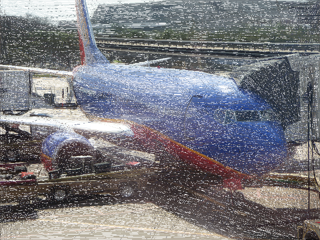
\includegraphics[width=2.3cm]{figs/thumb_threaded.png}};
\node[lab] at (0,\yb-1.0) {thread image\\(the only input)};
\draw[flow] (in.east) to[out=0, in=180] (3.3,\ya);
\draw[flow] (in.east) -- (3.3,\yb);
\draw[flow] (in.east) to[out=0, in=180] (3.3,\yc);

% ------------------------------------------------------------ VLM row
\node[title] (t1) at (3.3,\ya+1.5) {VLM};
\node[sub] at ($(t1.east)+(0.1,0)$) {Claude Opus 5.5, used as is};
\node[inner sep=0] (patch) at (4.4,\ya) {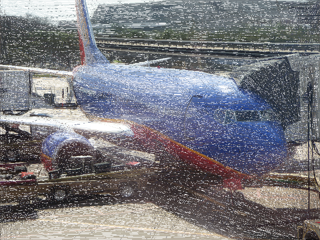
\includegraphics[width=\tw]{figs/thumb_threaded.png}};
\foreach \i in {1,2,3} \draw[white, line width=1.1pt] ($(patch.south west)!\i/4!(patch.south east)$) -- ($(patch.north west)!\i/4!(patch.north east)$);
\foreach \i in {1,2} \draw[white, line width=1.1pt] ($(patch.south west)!\i/3!(patch.north west)$) -- ($(patch.south east)!\i/3!(patch.north east)$);
\node[lab] at (4.4,\ya+\lb) {cut into patches};
\draw[flow] (patch.east) -- (6.0,\ya);
\draw[flow] (6.75,\ya) -- (7.05,\ya);
\draw[flow] (8.75,\ya) -- (9.35,\ya);

\pic at (6.05,\ya,0) {Box={name=venc, caption=, fill=okSky!70, opacity=1, height=12, width={1.2,1.2,1.2}, depth=12, scale=0.1}};
\node[lab] at (6.4,\ya+\lb) {vision\\encoder};
\foreach \i in {0,...,5} \node[draw=black!60, fill=okSky!70, minimum size=0.2cm, inner sep=0] at (7.25+0.28*\i,\ya) {};
\node[lab] at (7.95,\ya+\lb) {image\\tokens};
\node[card, font=\scriptsize\itshape] (prompt) at (7.95,\ya+0.8) {prompt:\\``name every object''};
\draw[flow] (prompt.south) -- (7.95,\ya+0.18);
\pic at (9.4,\ya,0) {Box={name=llm, caption=, fill=okBlue!45, opacity=1, height=13, width={1.6,1.6,1.6,1.6}, depth=13, scale=0.1}};
\node[lab] at (9.85,\ya+\lb) {language\\model};
\node[card, font=\scriptsize] (vout) at (\outx,\ya) {\texttt{airplane | truck |}\\\texttt{person | jet bridge}};
\draw[flow] (10.4,\ya) -- (vout.west);
\node[lab] at (\outx,\ya+\lb) {object names};

% ------------------------------------------------------------ YOLO row
\node[title] (t2) at (3.3,\yb+1.5) {YOLO};
\node[sub] at ($(t2.east)+(0.1,0)$) {YOLOv12n, used as released};
\draw[flow] (3.3,\yb) -- (3.6,\yb);
\draw[flow] (4.0,\yb) -- (4.55,\yb);
\draw[flow] (4.95,\yb) -- (5.5,\yb);
\draw[flow] (5.9,\yb) -- (6.45,\yb);
\draw[flow] (6.75,\yb) -- (7.55,\yb);

\pic at (3.65,\yb,0) {Box={name=b1, caption=, fill=okOrange!35, opacity=1, height=13, width=1.2, depth=13, scale=0.1}};
\pic at (4.6,\yb,0) {Box={name=b2, caption=, fill=okOrange!50, opacity=1, height=10, width=1.6, depth=10, scale=0.1}};
\pic at (5.55,\yb,0) {Box={name=b3, caption=, fill=okOrange!65, opacity=1, height=7, width=2.0, depth=7, scale=0.1}};
\pic at (6.5,\yb,0) {Box={name=b4, caption=, fill=okOrange!80, opacity=1, height=4.5, width=2.4, depth=4.5, scale=0.1}};
\node[lab] at (5.25,\yb+\lb) {convolutional layers\\(image shrinks, features grow)};
\pic at (7.6,\yb,0) {Box={name=head, caption=, fill=okVermillion!40, opacity=1, height=10, width={1.2,1.2,1.2}, depth=10, scale=0.1}};
\node[lab] at (8.0,\yb+\lb) {detection\\head};
\node[inner sep=0] (yout) at (\outx,\yb) {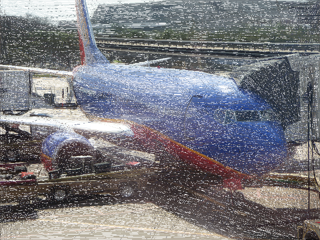
\includegraphics[width=\tw]{figs/thumb_threaded.png}};
% schematic boxes, kept inside the thumbnail
\draw[okVermillion, very thick] ($(yout.south west)+(0.30,0.42)$) rectangle ($(yout.north east)+(-0.15,-0.28)$);
\node[fill=okVermillion, text=white, font=\tiny, inner sep=1pt, anchor=north west] at ($(yout.north west)+(0.30,-0.28)$) {airplane};
\draw[okBlue, very thick] ($(yout.south west)+(0.05,0.05)$) rectangle ($(yout.south west)+(0.85,0.50)$);
\node[fill=okBlue, text=white, font=\tiny, inner sep=1pt, anchor=south west] at ($(yout.south west)+(0.05,0.05)$) {truck};
\draw[flow] (8.15,\yb) -- (yout.west);
\node[lab] at (\outx,\yb+\lb) {boxes with classes};

% ------------------------------------------------------------ human row
\node[title] (t3) at (3.3,\yc+1.2) {Human raters};
\node[sub] at ($(t3.east)+(0.1,0)$) {three raters, results to be added};
\fill[okGreen!70!black] (3.85,\yc+0.2) circle (0.15);
\fill[okGreen!70!black] (3.55,\yc-0.4) .. controls (3.55,\yc+0.05) and (4.15,\yc+0.05) .. (4.15,\yc-0.4) -- cycle;
\node[card, font=\scriptsize, text width=4.3cm] (hui) at (7.4,\yc) {web app: one image at a time,\\answers typed freely, no list of classes};
\draw[flow] (4.3,\yc) -- (hui.west);

\node[card, font=\scriptsize] (hout) at (\outx,\yc) {\texttt{plane | truck | worker}};
\draw[flow] (hui.east) -- (hout.west);
\node[lab] at (\outx,\yc-0.45) {object names};

% ------------------------------------------------------------ how each row is scored
\node[score, anchor=west] (s1) at (\outx+2.05,\ya) {mapped to\\COCO classes,\\scored by recall};
\node[score, anchor=west] (s2) at (\outx+2.05,\yb) {mapped to\\COCO classes,\\scored by recall};
\node[score, anchor=west] (s3) at (\outx+2.05,\yc) {mapped to\\COCO classes,\\scored by recall};
\draw[flow, dashed] (vout.east) -- (s1.west); \draw[flow, dashed] (yout.east) -- (s2.west); \draw[flow, dashed] (hout.east) -- (s3.west);
\end{tikzpicture}
